\chapter{Data Compression}
In this chapter we investigate how a given string can be stored so that the amount of memory used to store the
string is minimized.   We assume that a set of characters $\Sigma$ is given and that the string $s$ is a finite
sequence of characters from $\Sigma$, i.e.~$s \in \Sigma^*$.  The set of characters $\Sigma$ is called the
\blue{alphabet}.  If the alphabet $\Sigma$ contains $k$ different characters and if we use the same number of
bits $b$ for every character in $\Sigma$, then the number $b$ of bits must satisfy the inequality
\\[0.2cm]
\hspace*{1.3cm}
$\ds k \leq 2^b$,
\\[0.2cm]
which entails that 
\\[0.2cm]
\hspace*{1.3cm}
$b \geq \mathtt{ceil}\bigl(\log_2(k)\bigr)$
\\[0.2cm]
holds.  Here, $\mathtt{ceil}(x)$ denotes the
\href{https://en.wikipedia.org/wiki/Floor_and_ceiling_functions}{ceiling function}.  Given a real number $x$,
the expression $\mathtt{ceil}(x)$ returns the samllest integer $k$ that is as least as big as $x$, i.e.~we have
\\[0.2cm]
\hspace*{1.3cm}
$\mathtt{ceil}(x) = \min \{ k \in \mathbb{Z} \mid x \leq k \}$. 
\\[0.2cm]
If the string $s$ has a length of $m$ characters, then we have to use $m \cdot b$ bits in order to code $s$. 
There are two options to improve on this number.
\begin{enumerate}
\item If we drop the requirement to store all characters with the same amount of bits, then we can save some space.
      The idea is to code characters occurring very frequently with fewer than $b$ bits while those characters
      that are very rare are encoded using more than $b$ bits.  This approach leads to 
      \href{https://en.wikipedia.org/wiki/Huffman_coding}{Huffman's algorithm} that was discovered 1952 by 
      \href{https://en.wikipedia.org/wiki/David_A._Huffman}{David A.~Huffman (1925 -- 1999)} \cite{huffman:52}.
\item Alternatively we can try to extend the alphabet by interpreting substrings that occur very frequently as
      new letters.  For example, given an English text $s$, it is quite likely that the substring 
      ``\emph{the}'' occurs several times in $s$.  If this substring is then coded as a single new character,
      we might save some space.  The 
      \href{https://en.wikipedia.org/wiki/Lempel-Ziv-Welch}{Lempel-Ziv-Welch algorithm} 
      \cite{ziv:77,ziv:78,welch:84} was published in 1984 and is based on this idea.

\end{enumerate}
This chapter discusses both Huffman's algorithm and the Lempel-Ziv-Welch algorithm.

\section[Motivation]{Motivation of  Huffman's Algorithm \label{sec:huffman}}
The main idea of the
algorithm developed by Huffman is that letters that occur very frequently are encoded with
as few bits as possible, while letters that occur only rarely can be encoded with more bits. 
To clarify this idea we use the following example:  Assume our alphabet $\Sigma$ contains just four characters, we have
\\[0.2cm]
\hspace*{1.3cm}
$\Sigma = \{ \mathtt{a}, \mathtt{b}, \mathtt{c}, \texttt{d} \}$. 
\\[0.2cm]
The string $s \in \Sigma^*$ that is to be encoded is assumed to contain the letter
``\texttt{a}'' $990$ times, the letter ``\texttt{b}'' occurs $8$ times and the letters ``\texttt{c}'' and
``\texttt{d}'' each occur once.  Therefore, the string $s$ has a length of $1\,000$ characters.
If we encode each letter with $2 = \log_2(4)$ bits, then we need a total of $2\,000$ bits to store the string $s$.
We will now see that it is possible the store the string $s$ with less than $2\,000$ bits.
In our example, the character \texttt{a} occurs much more frequently that the other characters.  Therefore, we
encode ``\texttt{a}'' with a single bit.  On the other hand, the characters ``\texttt{c}'' and ``\texttt{d}''
each occur only once.  Therefore, it does no harm if we need more than two bits to encode these characters.
Table \ref{tab:coding} shows an encoding of the characters in $\Sigma$ that is based on these considerations.

\begin{table}[htbp]
  \centering
\begin{tabular}[t]{|l|r|r|r|r|}
\hline
Character  & \texttt{a} & \texttt{b}  & \texttt{c}   & \texttt{d}   \\
\hline
\hline
Frequency &     990    &         8   &           1  &         1    \\
\hline
Encoding  & \texttt{0} & \texttt{10} & \texttt{110} & \texttt{111} \\
\hline
\end{tabular}
  \caption{Variable-length encoding of the characters.}
  \label{tab:coding}
\end{table}
In order to understand how this encoding works we depict this encoding in Figure
 \ref{fig:coding-tree} as a  \blue{coding tree}:  The inner nodes of this tree do not contain any attributes
 and are therefore depicted as empty circles.  The leaves of this tree are labelled with characters.
The encoding of a character is given by the labelling of the edges that lead from the root of the tree to the
leaf containing that character.  For example, there is an edge from the root of this tree to the leaf labelled
with the digit ``\texttt{0}''.  Hence, the character ``\texttt{a}'' is encoded by the bit string ``\texttt{0}''.
To give another example we take the character ``\texttt{c}''.   The path that starts at the root and leads to
the leaf labelled with ``\texttt{c}'' consists of three edges.  The first two of these edges are labelled with
the bit ``\texttt{1}'', while the last edge is labelled with the bit ``\texttt{0}''.  Therefore, the character
 ``\texttt{c}'' is encoded by the bit string ``\texttt{110}''.

If we now encode the string $s$ that is made up from  $990$ occurrences of the character
``\texttt{a}'', $8$ occurrences of the character ``\texttt{b}'' and a single occurrence of both ``\texttt{c}''
and ``\texttt{d}'', then we need
\\[0.2cm]
\hspace*{1.3cm}
$990 \cdot 1 + 8 \cdot 2 + 1 \cdot 3 + 1 \cdot 3 = 1\,012$
\\[0.2cm]
bits if we use the variable length encoding shown in Figure \ref{fig:coding-tree}.  Comparing this to the fixed
width encoding that uses 2 bits per character and therefore uses $2\,000$ bits to store $s$, we see that we can
save $49,4\%$ of the bits with the variable length encoding shown in Table \ref{tab:coding}.

\begin{figure}[!ht]
  \centering
  \framebox{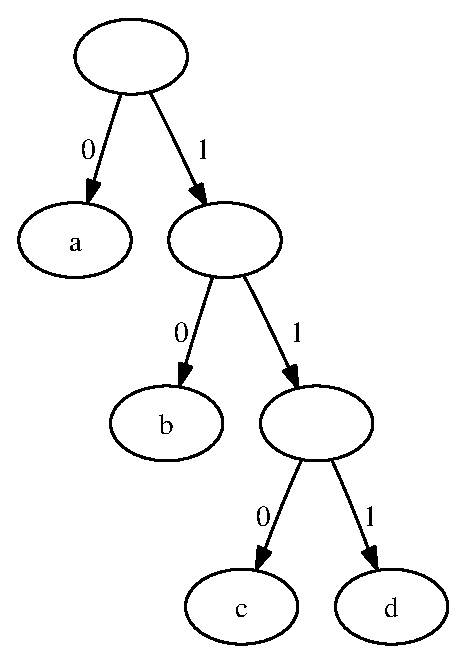
\epsfig{file=Abbildungen/coding-tree.eps, scale=0.5}} 
  \caption{Tree representation of the encoding shown in Figure \ref{tab:coding}.}
  \label{fig:coding-tree}
\end{figure}
In order to see how a bit string can be decoded using the encoding shown in Figure \ref{fig:coding-tree}
we consider the bit string ``\texttt{100111}''.  We start with the bit ``\texttt{1}'' which commands us to take
the right edge from the root of the coding tree.  Next, the bit ``\texttt{0}'' specifies the left edge.  
After following this edge we arrive at the leaf labelled with the character ``\texttt{b}''.  Hence we have
found the first character.  To decode the next character, we return to the root of the tree.  The edge labelled
``\texttt{0}'' takes us to the leaf labelled with the character ``\texttt{a}''.  Hence, we have found the
second character.  Again, we return to the root of the tree.  Now the bits ``\texttt{111}'' lead us to the
character ``\texttt{d}''.  This ends the decoding of the given bit string and we have therefore found that this
bit string encodes the string ``\texttt{bad}'', i.e.~we have
\\[0.2cm]
\hspace*{1.3cm}
``\texttt{100111}'' $\simeq$ ``\texttt{bad}''.


\section{Huffman's Algorithm}
Suppose we have been given a string $s \in \Sigma^*$ where $\Sigma$ is some alphabet.  How do we find an encoding of the letters such 
that the encoding of $s$ is as short as possible?  Huffman's algorithm answers this question.  In order 
to present this algorithm, we first define the set $\mathcal{K}$ of \blue{coding trees} by induction.
\begin{enumerate}
\item $\texttt{Leaf}(c,f) \in \mathcal{K} \quad \mbox{if $c \in \Sigma$ and $f \in \N$}$.

      An expression of the form $\texttt{Leaf}(c,f)$ represent a leaf in a coding tree.  Here  $c$ is a letter
      from the alphabet $\Sigma$ and $f$ is the number of times that the letter $c$ occurs in the string $s$
      that is to be encoded.

      Compared to Figure \ref{fig:coding-tree} this representation adds the frequency $f$ of the letters.
      This frequency information is needed since we intend to code frequent letters with fewer bits.
\item $\texttt{Node}(l,r) \in \mathcal{K} \quad \mbox{if $l \in\mathcal{K}$ and $r \in \mathcal{K}$.}$ 

      The expressions $\texttt{Node}(l,r)$ represent the inner nodes of the coding-tree.
\end{enumerate}
Next, we define the function
\\[0.2cm]
\hspace*{1.3cm}
$\texttt{count} : \mathcal{K} \rightarrow \N$.
\\[0.2cm] 
This function computes the sum of all frequencies of all letters occurring in a given coding tree.
\begin{enumerate}
\item For a leaf, the definition of $\texttt{count}$ is obvious:
      \\[0.2cm]
      \hspace*{1.3cm}
      $\texttt{Leaf}(c,f).\texttt{count}() = f$.
\item The sum of all frequencies of a coding tree of the form $\texttt{Node}(l,r)$ is the sum of all frequencies
      in $l$ plus the frequencies in $r$.  Therefore we have
      \\[0.2cm]
      \hspace*{1.3cm}
      $\texttt{Node}(l,r).\texttt{count}() = l.\texttt{count}() + r.\texttt{count}()$. 
\end{enumerate}
Next we define the function
\\[0.2cm]
\hspace*{1.3cm}
$\texttt{cost}: \mathcal{K} \rightarrow \N$.
\\[0.2cm]
The function $\texttt{cost}$ computes the number of bits that are necessary to encode a string $s$ if 
all letters occurring in $s$ occur in the the coding tree and if, furthermore, the frequencies of the letters
in $s$ are given by the frequencies stored in the coding tree.
The definition of $\texttt{cost}(t)$ is given by induction on the coding tree $t$.
\begin{enumerate}
\item $\texttt{Leaf}(c,f).\texttt{cost}() = 0$.

      As long as the coding tree has no edges, the resulting encoding has zero bits.
\item $\texttt{Node}(l,r).\texttt{cost}() = 
       l.\texttt{cost}() + r.\texttt{cost}() + l.\texttt{count}() + r.\texttt{count}()$.

      If two coding trees $l$ and $r$ are combined into a new coding tree, the encoding of all letters
      occurring in either $l$ or $r$ grows by one bit:  The encoding of a letter in $l$ is prefixed with the
      bit ``$0$'', while the encoding of a letter from $r$ is prefixed with the bit ``$1$''.  The sum
      \\[0.2cm]
      \hspace*{1.3cm}
      $l.\texttt{count}() + r.\texttt{count}()$
      \\[0.2cm] 
      counts the frequencies of all letters occurring in the coding tree.
      As the encoding of all these letters is lengthened by one bit,
      we have to add the term $l.\texttt{count}() + r.\texttt{count}()$ to the costs of $l$ and $r$.
\end{enumerate}
The function  $\texttt{cost}()$ is extended to sets of coding trees.  If $M$ is a set of coding trees, then we
define
\\[0.2cm]
\hspace*{1.3cm}
$\texttt{cost}(M) := \sum\limits_{n\in M} n.\texttt{cost}()$. 
\\[0.2cm]
The algorithm that was published by David A.~Huffman in 1952 \cite{huffman:52} starts with a set of pairs of
the form $\langle c, f\rangle$ where $c$ is a letter and $f$ is the frequency of this letter on a given string
$s$ that is to be encoded.  In the first step of this algorithm, these pairs are turned into leaves of a coding tree.
Assume that the string $s$ is built from the  letters
\\[0.2cm]
\hspace*{1.3cm}
$c_1$, $c_2$, $\cdots$, $c_k$
\\[0.2cm]
and that the frequencies of theses letters are givens as
\\[0.2cm]
\hspace*{1.3cm}
$f_1$, $f_2$, $\cdots$, $f_k$.
\\[0.2cm]
Then the set of coding trees is given as
\begin{equation}
  \label{eq:huffmann1}
 M = \bigl\{  \texttt{Leaf}(c_1, f_1), \cdots, \texttt{Leaf}(c_k, f_k) \bigr\}.   
\end{equation}
Huffmann's algorithm combines two nodes $a$ and $b$ from $M$ into a new node
$\texttt{Node}(a,b)$ until the set $M$ contains just a single node.  When combining the nodes of $M$ into a single
tree we have to take care that the cost of the resulting tree should be minimal.
Huffman's algorithm takes a \href{https://en.wikipedia.org/wiki/Greedy_algorithm}{greedy} approach: 
The idea is to combine those nodes $a$ and $b$ such that the cost of the set
\\[0.2cm]
\hspace*{1.3cm}
$M \symbol{92} \{a,b\} + \{ \texttt{Node}(a,b) \}$
\\[0.2cm]
is as small as possible.
In order to choose $a$ and $b$ let us investigate how much the cost increases if we combine the two nodes
into the new node $\texttt{Node}(a,b)$:
\begin{eqnarray*}
& & \texttt{cost}\bigl(N \cup \{ \texttt{Node}(a,b) \}\bigr) - \texttt{cost}\bigl(N \cup \{ a,b \}\bigr) \\
&=& \texttt{cost}\bigl( \{ \texttt{Node}(a,b) \}\bigr) - \texttt{cost}\bigl(\{ a,b \}\bigr)              \\
&=& \texttt{Node}(a,b).\texttt{cost}() - a.\texttt{cost}() - b.\texttt{cost}()                           \\
&=&   a.\texttt{cost}() + b.\texttt{cost}() + a.\texttt{count}() + b.\texttt{count}() 
    - a.\texttt{cost}() - b.\texttt{cost}()                                                              \\
&=& a.\texttt{count}() + b.\texttt{count}() 
\end{eqnarray*}
We see that if we combine $a$ and $b$ into the new node $\texttt{Node}(a,b)$, the cost is increased by the sum 
\\[0.2cm]
\hspace*{1.3cm}
$a.\texttt{count}() + b.\texttt{count}()$. 
\\[0.2cm]
If our intention is to keep the cost small then it suggests itself to pick those nodes
$a$ and $b$ from $M$ that have the smallest count and replace them with the new node
$\texttt{Node}(a,b)$.  This process is then iterated until the set $M$ contains but a single node.
It can be shown that this procedure yields a coding tree that codes the given string using the smallest number
of bits. 

\begin{figure}[!ht]
\centering
\begin{Verbatim}[ frame         = lines, 
                  framesep      = 0.3cm, 
                  labelposition = bottomline,
                  numbers       = left,
                  numbersep     = -0.2cm,
                  xleftmargin   = 1.3cm,
                  xrightmargin  = 1.3cm,
                ]
    codingTree := procedure(M) {
        while (#M > 1) {
            a := first(M);
            M -= { a };
            b := first(M);
            M -= { b };
            M += { [ a[1] + b[1], @Node(a, b) ] };
        }
        return arb(M);
    };
\end{Verbatim}
\vspace*{-0.3cm}
\caption{Huffman's algorithm implemented in \textsc{SetlX}.}
\label{fig:huffman.stlx}
\end{figure} 

\noindent
The function $\texttt{codingTree}$ program shown in Figure \ref{fig:huffman.stlx} implements this algorithm.
\begin{enumerate}
\item The function $\texttt{codingTree}$ is called with a set  $M$ of nodes.  This set has the form
      \\[0.2cm]
      \hspace*{1.3cm}
      $M = \bigl\{ [ f_1, \texttt{Leaf}(c_1) ], \cdots, [f_k, \texttt{Leaf}(c_k)] \bigr\}$.
      \\[0.2cm]
      Here, $c_1$, $\cdots$, $c_k$ are the different character that occur in the string $s$ that is to be encoded. 
      For every character $c_i$, the number $f_i$ counts the number of times that $c_i$ occurs in the string $s$.

      In the pairs $[f_i, \texttt{Leaf}(c_i)]$ the frequency $f_i$ is stored first.
      As \textsc{SetlX} stores this set internally as an ordered binary tree that is sorted ascendingly, this
      fact enables us to extract the node with the lowest frequency by calling the function $\texttt{first}$.
      The reason is that in \textsc{SetlX} pairs of the form $[f, \texttt{Leaf}(c)$ are compared
      lexicographically:  In order to compare two pairs
      \\[0.2cm]
      \hspace*{1.3cm}
      $[f_1, \texttt{Leaf}(c_1)]$ \quad and \quad $[f_2, \texttt{Leaf}(c_2)]$
      \\[0.2cm]
      \textsc{SetlX} first compares the frequencies $f_1$ and $f_2$.  If $f_1$ is less than $f_2$, the pair
      $[f_1, \texttt{Leaf}(c_1)]$ is considered to be smaller than $[f_2, \texttt{Leaf}(c_2)]$, if $f_2$ is bigger
      than $f_2$, then the pair $[f_1, \texttt{Leaf}(c_2)]$ is considered to be bigger than
      $[f_2,
      \texttt{Leaf}(c_2)]$.  Finally, if the frequencies $f_1$ and $f_2$ are the same, the characters $c_1$ and
      $c_2$ are compared to determine the order.  Hence, the first element of the set $M$ is the pair that has
      the smallest frequency.  Effectively, this trick turns the set $M$ into a priority queue:
      \begin{enumerate}
      \item The function $\texttt{first}$ that is predefined in \textsc{SetlX} returns the first element of the
            set $M$ and thus the call $\texttt{first}(M)$ achieves the same as the call $M.\texttt{top}()$
            would achieve if $M$ had been implemented as a priority queue.
      \item In order to insert an element $v$ with priority $v$ into $M$ we can use the expression
            \\[0.2cm]
            \hspace*{1.3cm}
            \texttt{$M$ += \{ [$p$, $v$] \};}
            \\[0.2cm]
            instead of writing $M.\texttt{insert}(p, v)$, which would have been necessary if $M$ had been
            implemented as a priority queue.
      \item In order to remove the top element from the priority queue $M$ we can use the expression
            \\[0.2cm]
            \hspace*{1.3cm}
            \texttt{$M$ -= \{ \texttt{first}($M$) \};}
            \\[0.2cm]
            This achieves the same effect as the call $M.\texttt{remove}()$ would have achieved if $M$ had been
            implemented as a priority queue.
      \end{enumerate}
      What makes this approach elegant is the fact that with this implementation all operations of the abstract
      data type \textsl{PrioQueue} have logarithmic complexity.  In the case of the operation
      $M.\texttt{top}()$ this is not optimal as the data structure heap achieves a constant complexity in this case.
      However, for every call of the form  $M.\texttt{top}()$ there is a call of the form
      $M.\texttt{remove}()$ and this call has a logarithmic complexity even if we implement the priority queue
      as a heap.   This complexity would dominate the overall complexity so that in the end the heap based
      implementation of the abstract data type \textsl{PrioQueue} has the same complexity as the set based
      implementation. 
\item The \texttt{while} loop in line 2 reduces the number of nodes of the set $M$ in every step by one.
      \begin{enumerate}
      \item Using the function $\texttt{first}()$, we compute those nodes $a$ and $b$ that have the lowest count.
      \item These two nodes are removed from $M$ .
      \item Next $a$ and $b$ are combined into the new node $\texttt{Node}(a,b)$ that is added to $M$.
      \end{enumerate}
\item The \texttt{while} loop terminates when $M$ contains but a single element.  This element
      is then extracted using the function $\texttt{arb}$ and is returned as the result.
\end{enumerate}
The running time of Huffman's algorithm is given as  $\Oh\bigl(n \cdot \ln(n)\bigr)$ where $n$ denotes the
number of different characters occurring in the string $s$.  The reason is that all
the operations inside the \texttt{while} loop have at most a logarithmic complexity in $n$ and the loop is
executed $n-1$ times.
 

\begin{table}[htbp]
  \centering
\begin{tabular}[t]{|l|r|r|r|r|r|}
\hline
Character  & \texttt{a} & \texttt{b} & \texttt{c} & \texttt{d} & \texttt{e} \\
\hline
\hline
Frequency &          1 &          2 &          3 &          4 &          5 \\
\hline
\end{tabular}
  \caption{Letters with their frequencies.}
  \label{tab:frequency}
\end{table}

We demonstrate Huffman's algorithm by computing  the coding tree that results from a string $s$ containing the
letters ``\texttt{a}'', ``\texttt{b}'', ``\texttt{c}'', ``\texttt{d}'', and ``\texttt{e}'' where the number of
occurrence of these letters are given in table \ref{tab:frequency} on page \pageref{tab:frequency}.
\begin{enumerate}
\item Initially, the set $M$ has the form
      \\[0.2cm]
      \hspace*{0.3cm}
      $ M = \bigl\{ \langle 1, \texttt{Leaf}(\texttt{a}) \rangle,\,
             \langle 2, \texttt{Leaf}(\texttt{b}) \rangle,\, 
             \langle 3, \texttt{Leaf}(\texttt{c}) \rangle,\,
             \langle 4, \texttt{Leaf}(\texttt{d}) \rangle,\,
             \langle 5, \texttt{Leaf}(\texttt{e}) \rangle\bigr\}. $
\item Apparently, the characters ``\texttt{a}'' and ``\texttt{b}'' occur with the lowest frequency.  Hence,
  these characters are removed from $M$ and instead the node 
      \\[0.2cm]
      \hspace*{0.3cm}
      $\texttt{Node}(\texttt{Leaf}(\texttt{a}), \texttt{Leaf}(\texttt{b}))$
      \\[0.2cm]
      is added to the set $M$.  The frequency of this new node is given as the sum of the frequencies of the
      characters ``\texttt{a}'' and ``\texttt{b}''.   Hence, the pair 
      \\[0.2cm]
      \hspace*{0.3cm}
      $\langle 3, \texttt{Node}\bigl(\texttt{Leaf}(\texttt{a}) \rangle, \texttt{Leaf}(\texttt{b}) \bigr) \rangle$
      \\[0.2cm]
      is inserted into the set  $M$.  The resulting form of $M$ is
      \\[0.2cm]
      \hspace*{0.3cm}
      $ \bigl\{\langle 3, \texttt{Leaf}(\texttt{c}) \rangle,\,
			\langle 3, \texttt{Node}(\texttt{Leaf}(\texttt{a}), \texttt{Leaf}(\texttt{b}))\rangle,\,
              \langle 4, \texttt{Leaf}(\texttt{d}) \rangle,\,
             \langle 5, \texttt{Leaf}(\texttt{e}) \rangle\bigr\}. $
\item The two pairs with the smallest frequencies are now
      \\[0.2cm]
      \hspace*{0.3cm}
      $ \langle 3, \texttt{Node}(\texttt{Leaf}(\texttt{a}), \texttt{Leaf}(\texttt{b})) \rangle \quad \mathrm{and} \quad \langle 3, \texttt{Leaf}(\texttt{c})\rangle$.
      \\[0.2cm]
      These pairs are removed form $M$ and replaced by 
      \\[0.2cm]
      \hspace*{0.3cm}
      $ \langle 6, \texttt{Node}(
           \texttt{Node}((\texttt{Leaf}(\texttt{a}), \texttt{Leaf}(\texttt{b})),\; 
           \texttt{Leaf}(\texttt{c}))\rangle$. 
      \\[0.2cm]
      Then $M$ is given as
      \\[0.2cm]
      \hspace*{0.3cm}
      $ \Bigl\{ 
        \langle 4, \texttt{Leaf}(\texttt{d}) \rangle,\;\langle 5, \texttt{Leaf}(\texttt{e}) \rangle,\;
        \langle 6, \texttt{Node}(
           \texttt{Node}(\texttt{Leaf}(\texttt{a}), \texttt{Leaf}(\texttt{b})),\; 
           \texttt{Leaf}(\texttt{c}))\Bigr\}. $
\item Now the pairs
      \\[0.2cm]
      \hspace*{0.3cm}
      $ \langle 4, \texttt{Leaf}(\texttt{d}) \rangle \quad \mathrm{and} \quad \langle 5, \texttt{Leaf}(\texttt{e}) \rangle$
      \\[0.2cm]
      are the pairs with the smallest frequency.
      We remove them and construct the new node \\[0.2cm]
      \hspace*{0.3cm}
      $\langle 9, \texttt{Node}(\texttt{Leaf}(\texttt{d}), \texttt{Leaf}(\texttt{e})) \rangle$.
      \\[0.2cm]
      This node is added to the set  $M$ and then $M$ is
      \\[0.2cm]
      \hspace*{0.3cm}
      $ \Bigl\{ 
        \langle 6, \texttt{Node}(
           \texttt{Node}(\texttt{Leaf}(\texttt{a}),
           \texttt{Leaf}(\texttt{b})),\,\texttt{Leaf}(\texttt{c},3))
        \rangle,\;
        \langle 9,\texttt{Node}(\texttt{Leaf}(\texttt{d},4), \texttt{Leaf}(\texttt{e},5)) \rangle
        \Bigr\}
           $.      
\item Now the set $M$ has just two elements.  These are combined into the single node 
      \\[0.2cm]
      \hspace*{0.3cm}
      $\texttt{Node}\biggl(
              \texttt{Node}\Bigl(
                 \texttt{Node}\bigl(\texttt{Leaf}(\texttt{a}), \texttt{Leaf}(\texttt{b})\bigr),\; 
                 \texttt{Leaf}(\texttt{c})\Bigr),\;
              \texttt{Node}\bigl(\texttt{Leaf}(\texttt{d}), \texttt{Leaf}(\texttt{e})\bigr)
         \biggr)
      $.
      \\[0.2cm]
      This node is our result.  Figure 
      \ref{fig:coding-tree2} shows the corresponding coding tree.  Here every node $n$ is labelled with its
      count.  The resulting encoding is shown in table  \ref{tab:coding2}.
\end{enumerate}

\begin{figure}[!ht]
  \centering
  \framebox{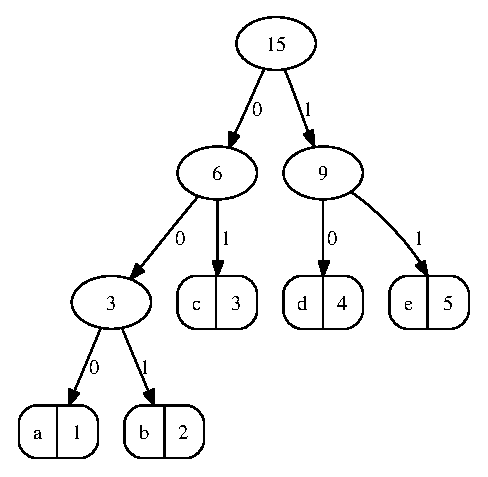
\epsfig{file=Abbildungen/coding-tree2.eps, scale=0.7}} 
  \caption{Tree representation of the coding tree.}
  \label{fig:coding-tree2}
\end{figure}



\begin{table}[htbp]
  \centering
\begin{tabular}[t]{|l|r|r|r|r|r|}
\hline
Character &   \texttt{a} &   \texttt{b} & \texttt{c}  & \texttt{d}  & \texttt{e}   \\
\hline
\hline
Encoding & \texttt{000} & \texttt{001} & \texttt{01} & \texttt{10} & \texttt{11} \\
\hline
\end{tabular}
  \caption{Variable length encoding of the letters ``\texttt{a}'' to ``\texttt{e}''.}
  \label{tab:coding2}
\end{table}
\pagebreak

\exercise
\begin{enumerate}[(a)]
\item Compute the Huffman code for a string $s$ that contains the letters 
      ``\texttt{a}'' through ``\texttt{g}'' where the frequencies are given by the following table:

\begin{table}[htbp]
  \centering
\begin{tabular}[t]{|l|r|r|r|r|r|r|r|}
\hline
Character  & \texttt{a} & \texttt{b} & \texttt{c} & \texttt{d} & \texttt{e} & \texttt{f} & \texttt{g} \\
\hline
\hline
Frequency &          1 &          1 &          2 &          3 &          5 &         8 &         13 \\
\hline
\end{tabular}
  \caption{Letters with frequencies.}
  \label{tab:aufgabe-huffman}
\end{table}

\item How many bits do we save when we use the Huffman encoding compared to a fixed with encoding?
\item Try to guess the law that has been used to specify the frequencies in the table given above
      and try to compute the Huffman code in the general case where the string $s$ has $n$ different
      characters. \eox
\end{enumerate}


\section[LZW Algorithm$^*$]{The Algorithm  of Lempel, Ziv, and Welch$^*$}
The algorithm developed by Abraham Lempel, Jacob Ziv \cite{ziv:77,ziv:78} and Terry A.~Welch
\cite{welch:84}, which is also known as the \blue{LZW algorithm}, is based on the idea that in most
texts certain combinations of letters are quite frequent.  Therefore, it should pay of to view
these combinations of letters as new letters and insert them into the alphabet.  This is the main
idea of the LZW algorithm.  However, since counting the occurrences of all words would be too time
consuming, the LZW algorithm works with a \blue{dynamic} coding dictionary.  Initially, this dictionary
contains only the \textsc{Ascii} characters.  Then, the idea is to extend this dictionary
dynamically: Every time a new string is encountered, it is entered into the dictionary and a code is
assigned to the corresponding string.  However, since it would not make sense to add arbitrary
strings to the dictionary, a new string $s$ of length $n=\#s$ is only added to the dictionary if
\begin{enumerate}
\item $s$ is a substring of the string that is encoded and
\item the substring $s[1..n-1]$ has already been entered into the dictionary.  
\end{enumerate} 
The algorithm is best
explained via an example.  The basic working of the algorithm is explained with the help of four
variables:
\begin{enumerate}
\item $\alpha$ is the last substring that has been encoded.  Initially, this is the empty string
      $\varepsilon$.
  
      The encoding of a string $s$ by the LZW algorithm works by encoding substrings of $s$ as
      numbers and $\alpha$ denotes the last of theses substrings.
\item $c$ is the next character of the string that is inspected.  This is also known as the
      \blue{look-ahead character}.
\item \textsl{d} is the dictionary mapping strings to numbers.  Initially, \textsl{d} maps all
      \textsc{Ascii} characters to their respective \textsc{Ascii} codes.
\item \texttt{nextCode} is the number assigned as code to the next string that is entered into
      the dictionary $d$.  Since the \textsc{Ascii} codes are the numbers from 0 up to 127,
      initially \texttt{nextCode} is equal to $128$.
\end{enumerate}
To describe the working of the algorithm, let us encode the string ``\texttt{maumau}''.
\begin{enumerate}
\item Initially, we have
      \\[0.2cm]
      \hspace*{1.3cm}
      $\alpha = \varepsilon$ \quad and \quad $c = \texttt{m}$.
      \\[0.2cm]
      Since the \textsc{Ascii} code of the character ``\texttt{m}'' is $109$, we output this number.
\item After reading the next character ``\texttt{a}'' we have
      \\[0.2cm]
      \hspace*{1.3cm}
      $\alpha = \texttt{m}$ \quad and \quad $c = \texttt{a}$.
      \\[0.2cm]
      Now, the substring $\alpha c$, which is ``\texttt{ma}'', is entered into the dictionary and
      assigned to the code $128$:
      \\[0.2cm]
      \hspace*{1.3cm}
      $d = d \cup \{\langle \texttt{ma}, 128 \rangle\}$.
      \\[0.2cm]
      Furthermore, we output the \textsc{Ascii} code of ``\texttt{a}'', which is $97$.
\item After reading the next character ``\texttt{u}'' we have
      \\[0.2cm]
      \hspace*{1.3cm}
      $\alpha = \texttt{a}$ \quad and \quad $c = \texttt{u}$.
      \\[0.2cm]
      Now, the substring $\alpha c$, which is ``\texttt{au}'', is entered into the dictionary and
      assigned to the next available code, which is $129$:
      \\[0.2cm]
      \hspace*{1.3cm}
      $d = d \cup \{\langle \texttt{au}, 129 \rangle\}$.
      \\[0.2cm]
      Furthermore, we output the \textsc{Ascii} code of ``\texttt{u}'', which is $117$.
\item After reading the next character, which is the character ``\texttt{m}'', we have
      \\[0.2cm]
      \hspace*{1.3cm}
      $\alpha = \texttt{u}$ \quad and \quad $c = \texttt{m}$.
      \\[0.2cm]
      Next, the substring $\alpha c$, which is ``\texttt{um}'', is entered into the dictionary and
      assigned to the next available code, which is $130$:
      \\[0.2cm]
      \hspace*{1.3cm}
      $d = d \cup \{\langle \texttt{um}, 130 \rangle\}$.
      \\[0.2cm]
      Since our dictionary already contains the substring ``\texttt{ma}'' and the character
      ``\texttt{a}'' is indeed the character following the character ``\texttt{m}'', we output
      $128$, which is the code assigned to the string ``\texttt{ma}''.

\item The next character to be read is now the final character ``\texttt{u}''.  We have
      \\[0.2cm]
      \hspace*{1.3cm}
      $\alpha = \texttt{ma}$ \quad and \quad $c = \texttt{u}$.
      \\[0.2cm]
      Next, the substring $\alpha c$, which is ``\texttt{mau}'', is entered into the dictionary and
      assigned to the next available code, which is $131$:
      \\[0.2cm]
      \hspace*{1.3cm}
      $d = d \cup \{\langle \texttt{mau}, 131 \rangle\}$.
      \\[0.2cm]
      Furthermore, we output the \textsc{Ascii} code of ``\texttt{u}'', which is $117$.
\end{enumerate} 
Putting everything together, we have coded the string ``\texttt{maumau}'' as the list
\\[0.2cm]
\hspace*{1.3cm}
$[109,97,117,128,117]$
\\[0.2cm]
If we had encoded this string in \textsc{Ascii} we would have used $6 \cdot 7 = 42$ bits.  Since the
dictionary that we have built on the fly uses codes starting at 128 we now have to use 8 bits to
encode the numbers.  However, we have only used 5 numbers to encode the string ``\texttt{maumau}''.
Hence we have only used $5 \cdot 8 = 40$ bits.   Of course, in this tiny example the compression
factor is quite low.  However, for texts that are longer and have more repetitions, the compression
factor is usually higher: On average, the experience shows that text corresponding to natural
language is compressed by a factor that is slightly bigger than $2$.

If we use the LZW algorithm there is no need to add the dictionary to the encoded string.  The
reason is that the recipient of an encoded string can construct the dictionary using exactly the
algorithm that is used when encoding the string.

Let us summarize the algorithm seen in the previous example:
\begin{enumerate}
\item The dictionary is initialized to map all \textsc{Ascii} characters to their \textsc{Ascii} codes.
\item Next, we search for the longest prefix $\beta$ of $s$ that is in the dictionary.  This prefix
      is removed from $s$.
\item We emit the code stored for $\beta$ in the dictionary.
\item Let $\alpha$ be the string that has been encoded in the previous step.  Append the first
      character $c$ of $\beta$ to $\alpha$ and enter the resulting string $\alpha c$ to the
      dictionary.

      This step expands the dictionary dynamically.
\item Go to step 2 and repeat as long as the string $s$ is not empty.
\end{enumerate}
Decoding a list of numbers $l$ into a string $s$ is quite similar to the encoding and works as follows.
\begin{enumerate}
\item This time, the dictionary is initialized to map all \textsc{Ascii} codes to their corresponding
      \textsc{Ascii} characters.  Hence, the dictionary constructed in this step is just the inverse
      of the dictionary constructed when starting to encode the string.
\item We initialize $s$ as the 
      empty string, which is denoted as $\varepsilon$:
      \\[0.2cm]
      \hspace*{1.3cm}
      $s := \varepsilon$.
\item We remove the first number $n$ from the list $l$ and look up the corresponding
      string $\beta$ in the dictionary.  This string is appended to $s$.
\item Assume that $\alpha$ is the string decoded in the previous iteration and that $c$ is the first
      character of $\beta$.  Enter the resulting string $\alpha c$ into the dictionary.
\item Goto step 2 and repeat as long as the list $l$ is not empty.
\end{enumerate}
The third step of this algorithm needs to refined:  The problem is
that it might happen that the dictionary does not have an entry for the number $n$.  This can occur because
the encoder is one step ahead of the decoder: The encoder encodes a substring and enters a code
corresponding to the previous substring into the dictionary.  Now if the next substring is identical
to the substring just entered, the encoder will produce a code that is not yet in the dictionary of
the decoder when he tries to decode it.   The question then is: How do we decode a number that has
not yet been entered into the dictionary.  To answer this question, we can reason as follows:
If the encoder outputs a code that it has just entered into the dictionary, then the string that is
encoded starts with the string that has been output previously, followed by some character.  However,
this character must be the first character of the string encoded now.  The string encoded now
corresponds to the code and hence this string is the same as the string previously decoded plus one
character. Therefore, if the previous string is $\alpha$, then the string
corresponding to an unknown code must be $\alpha \alpha[1]$, i.e. $\alpha$ followed by the first
character of $\alpha$.



\subsection{Implementing the LZW algorithm in \textsc{SetlX}}
In order to gain a better understanding of a complex algorithm it is best to code this algorithm.
Then the resulting program can be run on several examples.  Since humans tend
to learn better from examples than from logical reasoning, inspecting these examples deepens
the understanding of the algorithm.  We proceed to discuss an implementation of the LZW
algorithm.  

\begin{figure}[!ht]
\centering
\begin{Verbatim}[ frame         = lines, 
                  framesep      = 0.3cm, 
                  firstnumber   = 1,
                  labelposition = bottomline,
                  numbers       = left,
                  numbersep     = -0.2cm,
                  xleftmargin   = 0.8cm,
                  xrightmargin  = 0.8cm,
                ]
    class lzw() {
        mDictionary := { [ char(i), i ] : i in [32 .. 127] };
        mInverse    := { [ i, char(i) ] : i in [32 .. 127] };
        mNextCode   := 128;
    
        static {
            compress      := procedure(s)     { ... };
            uncompress    := procedure(l)     { ... };
            longestPrefix := procedure(s, i)  { ... };
        }
    }
\end{Verbatim}
\vspace*{-0.3cm}
\caption{Outline of the class \texttt{lzw}.}
\label{fig:lzw.stlx-outline}
\end{figure}


Figure \ref{fig:lzw.stlx-outline} shows the outline of the class \texttt{lzw}.  This class contains both the
method \texttt{compress} that takes a string $s$ and encodes this string into a list of numbers
and the method \texttt{uncompress} that takes a list of numbers $l$ and decodes this list back into
a string $s$.  These methods are designed to satisfy the following specification:
\\[0.2cm]
\hspace*{1.3cm}
$l = \texttt{lzw().compress}(s_1) \wedge s_2 = \texttt{lzw().uncompress}(l) \rightarrow s_1 = s_2$.
\\[0.2cm]
Furthermore, the class \texttt{lzw} contains the auxiliary method \texttt{longestPrefix}, which will
be discussed later.  The class \texttt{lzw} contains 3 member variables:
\begin{enumerate}
\item \texttt{mDictionary} is the dictionary used when encoding a string.  It is initialized to map
      the \textsc{Ascii} characters to their codes.  Remember that for a given number $i$, the
      expression $\texttt{char}(i)$ returns the \textsc{Ascii} character with code $i$.
\item \texttt{mInverse} is a binary relation that associates the codes with the corresponding
      strings.  It is initialized to map every number in the set $\{ 0, 1, 2, \cdots, 127 \}$
      with the corresponding \textsc{Ascii} character.  The binary relation \texttt{mInverse} is the
      inverse of the relation \texttt{mDictionary}.
\item \texttt{mNextCode} gives the value of the next code used in the dictionary.  Since the codes
      up to and including $127$ are already used for the \textsc{Ascii} character, the next
      available code will be $128$.
\end{enumerate}

\begin{figure}[!ht]
\centering
\begin{Verbatim}[ frame         = lines, 
                  framesep      = 0.3cm, 
                  firstnumber   = 1,
                  labelposition = bottomline,
                  numbers       = left,
                  numbersep     = -0.2cm,
                  xleftmargin   = 0.8cm,
                  xrightmargin  = 0.8cm,
                ]
    compress := procedure(s) {
        result := [];
        idx    := 1;
        while (idx <= #s) {
            p := longestPrefix(s, idx);
            result += [ mDictionary[s[idx..p]] ];
            if (p < #s) {
                mDictionary[s[idx..p+1]] := mNextCode;
                this.mNextCode += 1;
            }
            idx := p + 1;
        }
        return result;
    };
\end{Verbatim}
\vspace*{-0.3cm}
\caption{The method \texttt{compress} encodes a string as a list of integers.}
\label{fig:lzw.stlx-compress}
\end{figure}
Figure \ref{fig:lzw.stlx-compress} shows the implementation of the method compress.  We discuss this
implementation line by line.
\begin{enumerate}
\item The variable \texttt{result} points to the list that encodes the string $s$ given as argument.
      Initially, this list is empty.  Every time a substring of $s$ is encoded, the corresponding code
      is appended to this list.
\item The variable \texttt{idx} is an index into the string $s$.  The idea is that the substring
      $s[1..\texttt{idx}-1]$ has been encoded and the corresponding codes have already been written
      to the list \texttt{result}, while the substring $s[\texttt{idx}..]$ is
      the part of $s$ that still needs to be encoded.
\item Hence, the \texttt{while}-loop runs as long as the index \texttt{idx} is less or equal than
      the length $\texttt{\#}s$ of the string $s$.
\item Next, the method \texttt{longestPrefix}  computes the index of longest prefix of the substring
      $s[\texttt{idx}..]$ that can be found in the dictionary \texttt{mDictionary}, i.e.~$p$ is the
      maximal number such that the expression \texttt{mDictionary[s[idx..p]]} is defined.
\item The code corresponding to this substring is looked up in \texttt{mDictionary}
      and is then appended to the list \texttt{result}.
\item Next, we take care to maintain the dictionary \texttt{mDictionary} and add the substring
      $s[\texttt{idx}..p+1]$ to the dictionary.  Of course, we can only do this if the upper index
      of this expression, which is $p+1$, is an index into the string $s$. 
      Therefore we have to check that $p < \texttt{\#}s$.
      Once we have entered the
      new string with its corresponding code into the dictionary, we have to make sure that the
      variable \texttt{mNextCode} is incremented so that every string is associated with a unique
      code.  
\item Since the code corresponding to the substring $s[\texttt{idx}..p]$ has been written to the
      list \texttt{result}, the index \texttt{idx} is set to $p+1$.
\item Once the while loop has terminated, the string $s$ has been completely encoded and the list
      containing the codes can be returned.
\end{enumerate}


\begin{figure}[!ht]
\centering
\begin{Verbatim}[ frame         = lines, 
                  framesep      = 0.3cm, 
                  firstnumber   = 1,
                  labelposition = bottomline,
                  numbers       = left,
                  numbersep     = -0.2cm,
                  xleftmargin   = 0.8cm,
                  xrightmargin  = 0.8cm,
                ]
    longestPrefix := procedure(s, i) {
       oldK := i;
       k    := i+1;
       while (k <= #s && mDictionary[s[i..k]] != om) {
           oldK := k;
           k    += 1;
       }
       return oldK;
    };
    incrementBitNumber := procedure() {
        if (2 ** mBitNumber <= mNextCode) {
            this.mBitNumber += 1;
        }
    };
\end{Verbatim}
\vspace*{-0.3cm}
\caption{Computing the longest prefix.}
\label{fig:lzw.stlx-longestPrefix}
\end{figure}
Figure \ref{fig:lzw.stlx-longestPrefix} show the implementation of the auxiliary function
\texttt{longestPrefix}.  
The function $\texttt{longestPrefix}(s, i)$ computes the maximum value of $k$ such that
\\[0.2cm]
\hspace*{1.3cm}
$i \leq k \wedge k \leq \texttt{\#}s \wedge \texttt{mDictionary}[s[i..k]] \not= \Omega$.
\\[0.2cm]
This value is well defined since the dictionary is initialized to contain all strings of
length 1.  Therefore, $\texttt{mDictionary}[s[i..i]]$ is known to be defined: It is the
\textsc{Ascii} code of the character $s[i]$.
      
The required value is computed by a simple \texttt{while}-loop that tests all possible values of $k$.
The loop exits once the value of $k$ is too big.  Then the previous value of $k$, which is
stored in the variable \texttt{oldK} is returned as the result.




\begin{figure}[!ht]
\centering
\begin{Verbatim}[ frame         = lines, 
                  framesep      = 0.3cm, 
                  firstnumber   = 1,
                  labelposition = bottomline,
                  numbers       = left,
                  numbersep     = -0.2cm,
                  xleftmargin   = 0.8cm,
                  xrightmargin  = 0.8cm,
                ]
    uncompress := procedure(l) {
        result := "";
        idx    := 1;
        code   := l[idx]; 
        old    := mInverse[code];
        idx    += 1;
        while (idx < #l) {
            result += old;
            code := l[idx];
            idx  += 1;
            next := mInverse[code];
            if (next == om) {
                next := old + old[1];
            }
            mInverse[mNextCode] := old + next[1];
            this.mNextCode += 1;
            old := next;
        }
        result += old;
        return result;
    };
\end{Verbatim}
\vspace*{-0.3cm}
\caption{The method \texttt{uncompress} to decode a list of integers into a string.}
\label{fig:lzw.stlx-uncompress}
\end{figure}
Figure \ref{fig:lzw.stlx-uncompress} shows the implementation of the method \texttt{uncompress} that
takes a list of numbers and decodes it into a string $s$.
\begin{enumerate}
\item The variable \texttt{result} contains the decoded string.  Initially, this variable is empty.
      Every time a code of the list $l$ is deciphered into some string, this string is added to
      \texttt{result}.
\item The variable \texttt{idx} is an index into the list $l$.  It points to the next code that
      needs to be deciphered.
\item The variable \texttt{code} contains the code in $l$ at position \texttt{idx}.  Therefore, we
      always have
      \\[0.2cm]
      \hspace*{1.3cm}
      $l[\texttt{idx}] = \texttt{code}$
\item The variable \texttt{old} contains the substring associated with \texttt{code}.  Therefore,
      the invariant
      \\[0.2cm]
      \hspace*{1.3cm}
      $\texttt{mInverse}[\texttt{code}] = \texttt{old}$
      \\[0.2cm]
      is maintained.
\item As long as the index \texttt{idx} still points inside the list, the substring 
      that has just been decoded is appended to the string \texttt{result}.
\item Then, an attempt is made to decode the next number in the list $l$ by looking up the code
      in the dictionary \texttt{mInverse}.  
      
      Now there is one subtle case: If the \texttt{code} has not yet been defined in the
      dictionary,  then we can conclude that this code has been created when coding the
      substring \texttt{old} followed by some character $c$.  However, as the next substring $\beta$
      corresponds to this code, the character $c$ must be the first
      character of this substring, i.e.~we have
      \\[0.2cm]
      \hspace*{1.3cm}
      $c = \beta[1]$.
      \\[0.2cm]
      On the other hand, we know that the substring $\beta$ has the form
      \\[0.2cm]
      \hspace*{1.3cm}
      $\beta = \texttt{old} + c$,
      \\[0.2cm]
      where the operator ``$+$'' denotes string concatenation.  But then the first character of this string
      must be the first character of \texttt{old}, i.e.~we have
      \\[0.2cm]
      \hspace*{1.3cm}
      $\beta[1] = \texttt{old}[1]$
      \\[0.2cm]
      and hence we have shown that
      \\[0.2cm]
      \hspace*{1.3cm}
      $c = \texttt{old}[1]$.
      \\[0.2cm]
      Therefore, we conclude
      \\[0.2cm]
      \hspace*{1.3cm}
      $\beta = \texttt{old} + \texttt{old}[1]$
      \\[0.2cm]
      and hence this is the string encoded by a code that is not yet defined in the dictionary
      \texttt{mInverse}.
\item Next, we need to maintain the dictionary \texttt{mInverse} in the same fashion as the
      dictionary \texttt{mDictionary} is maintained in the method \texttt{compress}:
      Hence we take the string previously decoded and concat the next character of the
      string decoded in the current step.  Of course, this string is
      \\[0.2cm]
      \hspace*{1.3cm}
      $\texttt{old} + \texttt{next}[1]$
      \\[0.2cm]
      and this string is then associated with the next available code value.
\item At the end of the loop, we need to set \texttt{old} to \texttt{next} so that \texttt{old}
      will always contain the string decoded in the previous step.
\item When the \texttt{while}-loop has terminated, we still need to append the final value of \texttt{old}
      to the variable \texttt{result}.
\end{enumerate}
Now that we have discussed the implementation of the \texttt{LZW} algorithm I would like to
encourage you to test it on several examples that are not too long.  Time does not permit me
to discuss examples of this kind in these lecture notes and, indeed, I do not think that discussing
these examples here would be as beneficial for the student as performing the algorithm on their own.

\exercise
\begin{enumerate}[(a)]
\item Use the LZW algorithm to encode the string ``\texttt{abcabcabcabc}''.  Compute the compression
      factor for this string.
\item For all $n \in \mathbb{N}$ with $n \geq 1$ the string $\alpha_n$ is defined inductively as
      follows:
      \\[0.2cm]
      \hspace*{1.3cm} $\alpha_1 := \texttt{a}$ \quad and \quad $\alpha_{n+1} = \alpha_n + \texttt{a}$.
      \\[0.2cm]
      Hence, the string $\alpha_n$ has the form $\underbrace{\texttt{a} \cdots \texttt{a}}_n$,
      i.e. it is the character \texttt{a} repeated $n$ times.
      Encode the string $\alpha_n$ using the LZW algorithm.  What is the compression rate?
\item Decode the list 
      \\[0.2cm]
      \hspace*{1.3cm}
      $[97, 98, 128, 130]$
      \\[0.2cm]
      using the LZW algorithm.  \eox
\end{enumerate}

%%% Local Variables: 
%%% mode: latex
%%% TeX-master: "algorithms"
%%% End: 
